\documentclass[12pt]{article}
\usepackage{amssymb}
\usepackage{amsmath}
\usepackage{color}
\usepackage{graphicx}
\usepackage{mdframed}
\usepackage{listings, xcolor}
\usepackage{textcomp}

\definecolor{verylightgray}{rgb}{.97,.97,.97}
\definecolor{lightred}{rgb}{.97,.50,.50}

\lstdefinelanguage{myC}{
        keywords=[1]{break, case, continue, default, do
, else, false, for, if, const, return, switch, true, while}, % generic keywords
        keywordstyle=[1]\color{blue}\bfseries,
        keywords=[2]{bool, int, long, float, double, byte, short, char, void, signed, unsigned}, % types
        keywordstyle=[2]\color{teal}\bfseries,
        keywordstyle=[2]\color{violet}\bfseries,
        keywords=[3]{NULL},
        keywordstyle=[3]\color{teal}\bfseries,
        identifierstyle=\color{black},
        sensitive=false,
        comment=[l]{//},
        morecomment=[s]{/*}{*/},
        commentstyle=\color{violet}\ttfamily,
        commentstyle=\small\ttfamily\color{myGreen},
        stringstyle=\color{red}\ttfamily,
        morestring=[b]',
        morestring=[b]"
}

\lstset{
        language=myC,
        backgroundcolor=\color{verylightgray},
        extendedchars=true,
        basicstyle=\small\ttfamily,
        showstringspaces=false,
        showspaces=false,
        numbers=none,
        numberstyle=\small,
        numbersep=9pt,
        tabsize=2,
        upquote=true,
        breaklines=true,
        showtabs=false,
        captionpos=b
        otherkeywords={define,include,\# }
}

\definecolor{myBlue}{rgb}{0.5,0.5,1}
\definecolor{myLightBlue}{rgb}{0.35,0.6,0.8}
\definecolor{myBlack}{rgb}{0,0,0}
\definecolor{myGreen}{rgb}{0.1,0.6,0.2}
\definecolor{myGray}{rgb}{0.5,0.5,0.5}
\definecolor{myLightgray}{rgb}{0.95,0.95,0.95}
\definecolor{myMauve}{rgb}{0.58,0,0.82}
\lstdefinelanguage{customc}{
    language=C,
    backgroundcolor = \color{myLightgray},
    basicstyle=\small\ttfamily\color{myBlack},
    keywordstyle=\color{myLightBlue},
    keywordstyle=[2]\color{red},
    commentstyle=\small\ttfamily\color{myGreen},
    morekeywords={RequirePackage,ProvidesPackage},
    %
    % The special highlighting works for '!if', '!endif' and '!else'
    % But it doesn't work for '#if', '#endif' and '#else'.
    alsoletter = {!},
    keywords=[2]{!if,!endif,!else},
    otherkeywords={define,include,\# }
}

\lstdefinestyle{myCustomc}{
    language = customc,
    % keywordstyle = \color{myMauve},
}

\lstset{escapechar=@,style=myCustomc}


\definecolor{grey}{rgb}{0.3,0.3,0.3}
\definecolor{lightgrey}{rgb}{0.9,0.9,0.9}

\thispagestyle{empty}
\setlength{\textwidth}{18.5cm}
\setlength{\topmargin}{-2.5cm}
\setlength{\textheight}{24.5cm}
\setlength{\oddsidemargin}{-1cm}
\setlength{\evensidemargin}{-1cm}

\begin{document}
\begin{center}{\LARGE Compito di Programmazione I - Bioinformatica}\\
\begin{center}
  \large 13 settembre 2024 (tempo disponibile: 2 ore)
\end{center}
\end{center}

\vspace*{1ex}
\begin{center}{\Large Esercizio 1} ($15$ punti)\\
  \textbf{(si consegni \texttt{myatoi.c} e \texttt{myatoi.h})}
\end{center}

Si completi \texttt{myatoi.c}, completando la funzione
\texttt{myatoip(p,s)} in modo che restituisca
l'intero \texttt{long} ottenuto facendo seguire al
\texttt{long p} le cifre della stringa \texttt{s}, che si assume essere composta
solo da caratteri
tra il carattere dello \texttt{0} e il carattere del \texttt{9}, inclusi.
La funzione \texttt{myatoip}
deve essere ricorsiva. Per esempio, si dovr\`a avere:

\begin{mdframed}[backgroundcolor=verylightgray] 
\begin{verbatim}
myatoip(134, "3904") = 1343904
myatoip(1340, "3904") = 13403904
myatoip(22311, "0345895") = 223110345895
myatoip(0, "3458") = 3458
myatoip(13, "0") = 130
myatoip(13, "") = 13
\end{verbatim}
\end{mdframed}

Si completi quindi la funzione \texttt{myatoi(s)} in modo che restituisca
l'intero \texttt{long} corrispondente alla stringa \texttt{s}, che si assume essere
composta solo da caratteri tra il carattere dello \texttt{0} e il carattere del \texttt{9},
inclusi. La funzione \texttt{myatoi} deve essere implementata usando la funzione ausiliaria
\texttt{myatoip}.

Si scriva il file \texttt{myatoi.h} che dichiara solo la funzione \texttt{myatoi}.

Se tutto \`e corretto, compilando insieme a \texttt{main\_myatoi.c} (gi\`a scritto, da non
modificare) ed ese\-guendo il risultato, verr\`a stampato:

\begin{mdframed}[backgroundcolor=verylightgray] 
\begin{verbatim}
myatoi("12345") = 12345
myatoi("012345") = 12345
myatoi("54321") = 54321
myatoi("543210") = 543210
myatoi("192837465") = 192837465
myatoi("23344556678026") = 23344556678026
myatoi("") = 0
\end{verbatim}
\end{mdframed}

\textbf{Suggerimento:} per intuire il meccanismo ricorsivo di \texttt{myatoip}, si noti per
esempio che le seguenti uguaglianze sono vere:

\begin{mdframed}[backgroundcolor=verylightgray] 
\begin{verbatim}
myatoip(1340, "3904") = myatoip(13403, "904") = myatoip(134039, "04")
  = myatoip(1340390, "4") = myatoip(13403904, "") = 13403904
\end{verbatim}
\end{mdframed}

\vspace*{1ex}
\begin{center}{\Large Esercizio 2} ($16$ punti)\\
  \textbf{(si consegni \texttt{tokenizer.c})}
\end{center}
Un tokenizer è uno strumento di analisi del linguaggio naturale che divide una stringa in pezzetti (tokens) sulla base di un separatore o in base ad altri criteri.

Si modifichi opportunamente il file \texttt{tokenizer.c} in modo da costruire e stampare una lista di token a partire da una stringa che contiene i token separati da punto e virgola. 
In particolare, data in input una stringa del tipo \emph{"Alessandra;Jessica;Kaur;Francesca;Vittoria"} si deve costruire una lista di 5 nodi, esemplificata in Figura \ref{fig1}.
\begin{figure}
    \centering
    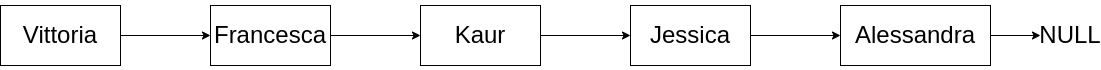
\includegraphics[width=0.8\linewidth]{es1.png}
    \caption{Esempio}
    \label{fig1}
\end{figure}
Si assuma che ogni token sia lungo al più \texttt{MAX$\_$LENGTH-1} caratteri.
Si noti che nell'esempio i token son inseriti sempre in testa alla lista; nell'implementazione si può scegliere liberamente se inserirli in testa o in coda.
\begin{mdframed}[backgroundcolor=myLightBlue] 
  \vspace*{-0.5ex}
  \textbf{La funzione main è gi\`a scritta e completa, non va modificata. Si possono aggiungere funzioni ausiliare in \texttt{tokenizer.c}. Attenzione, NON si può usare la funzione di libreria \texttt{strtok} di \texttt{string.h}.}
\end{mdframed}
%
\begin{lstlisting}[language=myC]
#include <stdio.h>
#define MAX_LENGTH 50
#define MAX_STRING_LENGTH 300
struct Nodo{
    //definizione di struttura da completare 
};

struct Nodo * mystrtok(char *s){
//da completare
}

void print_list(struct Nodo *l) {
//da completare
}

int caratteri_validi(char * elenco){	
//da completare
}

int main(void){
	char elenco_nomi[MAX_STRING_LENGTH];//ESEMPIO "Maria;Jessica;Kaur;Michela;Marco;Angelica;"
	int len = -1;
	
	do{
		printf("Inserisci un elenco di nomi, separati dal punto e virgola (;). La lunghezza complessiva deve essere inferiore a %d caratteri: ", MAX_STRING_LENGTH);	
		scanf("%s",elenco_nomi);

		len = strlen(elenco_nomi);
		
		if(!caratteri_validi(elenco_nomi) || len >= MAX_STRING_LENGTH) {
			printf("Errore nell'input, riprovare\n");
		}
	}	while(!caratteri_validi(elenco_nomi) || len >= MAX_STRING_LENGTH);
	
	struct Nodo* L=mystrtok(elenco_nomi);
	print_list(L);	
	return 0;
}	
\end{lstlisting}
In particolare si completino le funzioni:

\begin{itemize}
\item \texttt{mystrtok} che riceve in input una stringa formata da parole separate da punto e virgola e crea una lista dove ogni nodo contiene una di quelle parole. Quando si implementa la funzione \texttt{mystrtok}, SI DEVONO utilizzare i puntatori per scorrere la stringa ed estrarre i token. \textit{BONUS: Se un token supera la lunghezza massima \texttt{MAX$\_$LENGTH}, i caratteri in eccesso devono essere ignorati.}
\item \texttt{print$\_$list} che stampa una lista di token, stampando un token per ogni riga. 
\item \texttt{caratteri$\_$validi} che riceve in input una stringa e ritorna 1 se la stringa è formata da caratteri alfabetici ([A-Z] e [a-z]) e/o dal punto e virgola (';'), 0 altrimenti.
\end{itemize}

Se tutto \`e corretto, un esempio di esecuzione di \texttt{tokenizer.c}, specificando in input la stringa

\textit{Elena;Vittoria;Maria} \`e:
\begin{mdframed}[backgroundcolor=verylightgray] 
\begin{verbatim}
Maria
Vittoria
Elena
\end{verbatim}
\end{mdframed}
Si noti che anche ; è un input valido.


\end{document}

